\chapter {Interfacing a Light Emitting Diode}
\thispagestyle{empty}
\label{led}
\newcommand{\LocLEDfig}{\Origin/user-code/led/figures}
\newcommand{\LocLEDscicode}{\Origin/user-code/led/scilab}
\newcommand{\LocLEDscibrief}[1]{{\tt \seqsplit{%
        Origin/user-code/led/scilab/#1}}, see \fnrefp{fn:file-loc}}
\newcommand{\LocLEDardcode}{\Origin/user-code/led/arduino}
\newcommand{\LocLEDardbrief}[1]{{\tt \seqsplit{%
        Origin/user-code/led/arduino/#1}}, see \fnrefp{fn:file-loc}}

\newcommand{\LocLEDpycode}{\Origin/user-code/led/python}  %added for python
\newcommand{\LocLEDpybrief}[1]{{\tt \seqsplit{%
        Origin/user-code/led/python/#1}}, see \fnrefp{fn:file-loc}} % added for python


\newcommand{\LocLEDjuliacode}{\Origin/user-code/led/julia}  %added for julia
\newcommand{\LocLEDjuliabrief}[1]{{\tt \seqsplit{%
        Origin/user-code/led/julia/#1}}, see \fnrefp{fn:file-loc}} % added for julia

%%%%%%OpenModelica Starts
\newcommand{\LocLEDOpenModelicacode}{\Origin/user-code/led/OpenModelica}  %added for OpenModelica
\newcommand{\LocLEDOpenModelicabrief}[1]{{\tt \seqsplit{%
        Origin/user-code/led/OpenModelica/#1}}, see \fnrefp{fn:file-loc}} % added for OpenModelica

%%%%%OpenModelcia Ends

In this chapter, we will learn how to control the LEDs on the shield
and on the \arduino\ board.  We will do this through the Arduino IDE,
Scilab scripts, Scilab Xcos, Python, Julia, and OpenModelica.  
These are beginner level experiments,
and often referred to as the \emph{hello world} task of Arduino.
Although simple, controlling LED is a very important task in all
kinds of electronic boards.

\section{Preliminaries}
\label{sec:led-pril}
A light emitting diode (LED) is a special type of semiconductor diode,
which emits light when voltage is applied across its terminals. A
typical LED has 2 leads: Anode, the positive terminal and Cathode, the
negative terminal.  When sufficient voltage is applied, electrons
combine with the holes, thereby releasing energy in the form of
photons.  These photons emit light and this phenomenon is known as
electroluminescence.  The symbolic representation of an LED is shown
in \figref{fig:ledsym}.  Generally, LEDs are capable of emitting
different colours.  Changing the composition of alloys that are
present in LED helps produce different colours.  A popular LED is an
RGB LED that actually has three LEDs: red, green and blue.

\begin{figure}
  \centering
  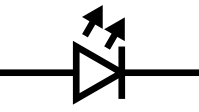
\includegraphics[width=0.2\linewidth]{\LocLEDfig/led.png}
  \caption{Light Emitting Diode}
  \label{fig:ledsym}
\end{figure}

%\subsection{Connection diagram}
An RGB LED is present on the shield provided in the kit.  In this
section, we will see how to light each of the LEDs present in the RGB
LED.  As a matter of fact, it is possible to create many colours by
combining these three.  A schematic of the RGB LED in the shield is
given in \figref{fig:ledblock}.
\begin{figure}
  \centering
  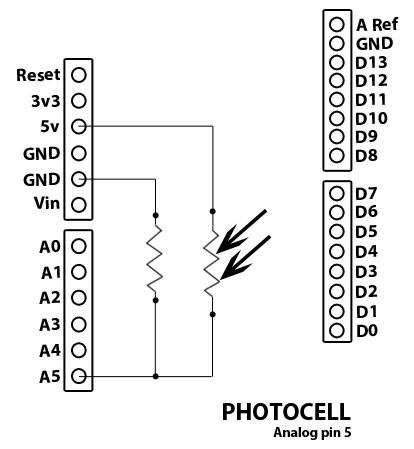
\includegraphics[width=\smfig]{\LocLEDfig/schematic.png}
  \caption{Internal connection diagram for LED on the shield}
  \label{fig:ledblock}
\end{figure}
The anode pins of red, green, and blue are connected to pins 11, 10, and 9, 
respectively. Common Cathode is connected to the ground.

It should be pointed out, however, that no wire connections are to be
made by the learner: all the required connections are already made internally 
and it is ready to use.  The LED of any colour can be turned on by
putting a high voltage on the corresponding anode pin.

\begin{figure}
  \centering
  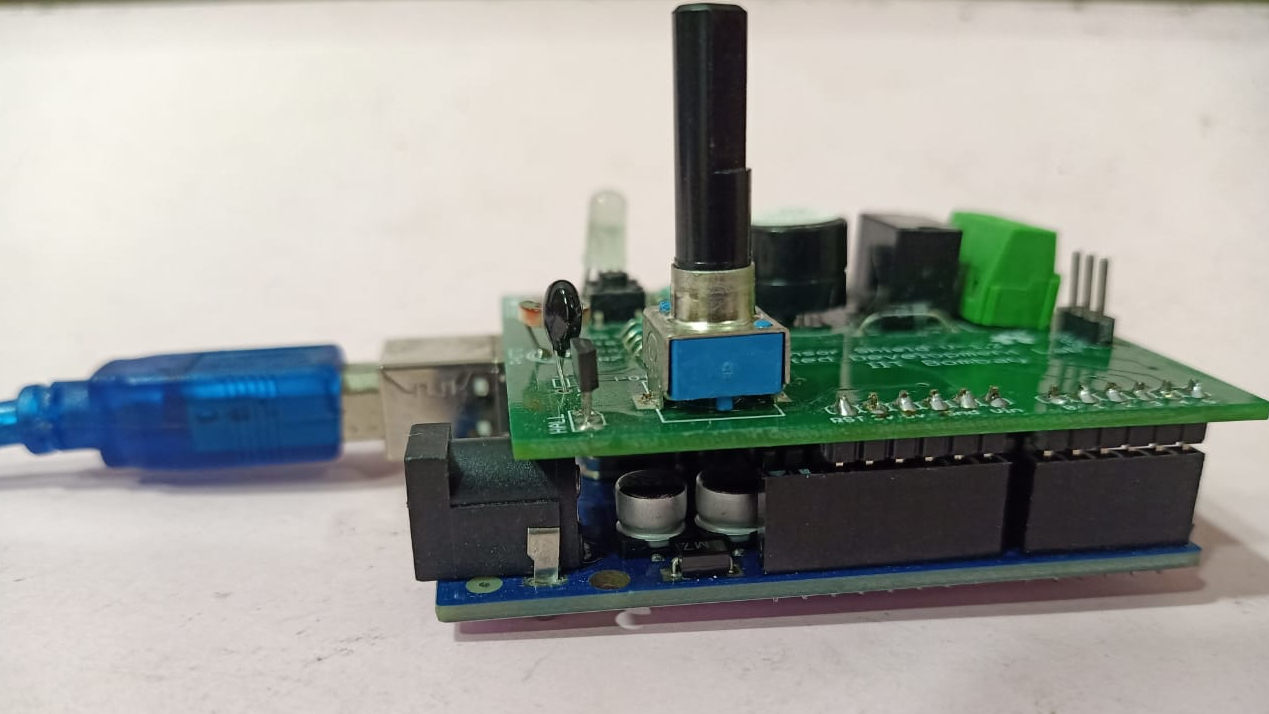
\includegraphics[width=\lgfig]{\LocLEDfig/arduino-new-shield.jpeg}
  \caption{Connecting \arduino\ and shield}
  \label{fig:uno-shield-connect}
\end{figure}

One should remember to connect the shield on to the \arduino\ board, as
shown in \figref{fig:uno-shield-connect}. All the experiments in this
chapter assume that the shield is connected to the \arduino\ board.
It is also possible to do some of the experiments without the shield,
which is pointed out in the next section. 

\section{Connecting an RGB LED with \arduino\ using a breadboard}
This section is useful for those who either don't have a shield or don't want to use the shield
for performing the experiments given in this chapter. 

A breadboard is a device for holding the components of a circuit and connecting 
them together. We can build an electronic circuit on a breadboard without doing any 
soldering. To know more about the breadboard and other electronic components, 
one should watch the Spoken Tutorials on Arduino as published on
{\tt https://spoken-tutorial.org/}. Ideally, one should go through all the
tutorials labeled as Basic. However, we strongly recommend the readers should
watch the fifth and sixth tutorials, i.e., {\tt First Arduino Program} and 
{\tt Arduino with Tricolor LED and Push button}.

In case you have an RGB LED and want to connect it with \arduino\ on a breadboard, 
please refer to \figref{fig:ard-rgb-bread}. 
\begin{figure}
  \centering
  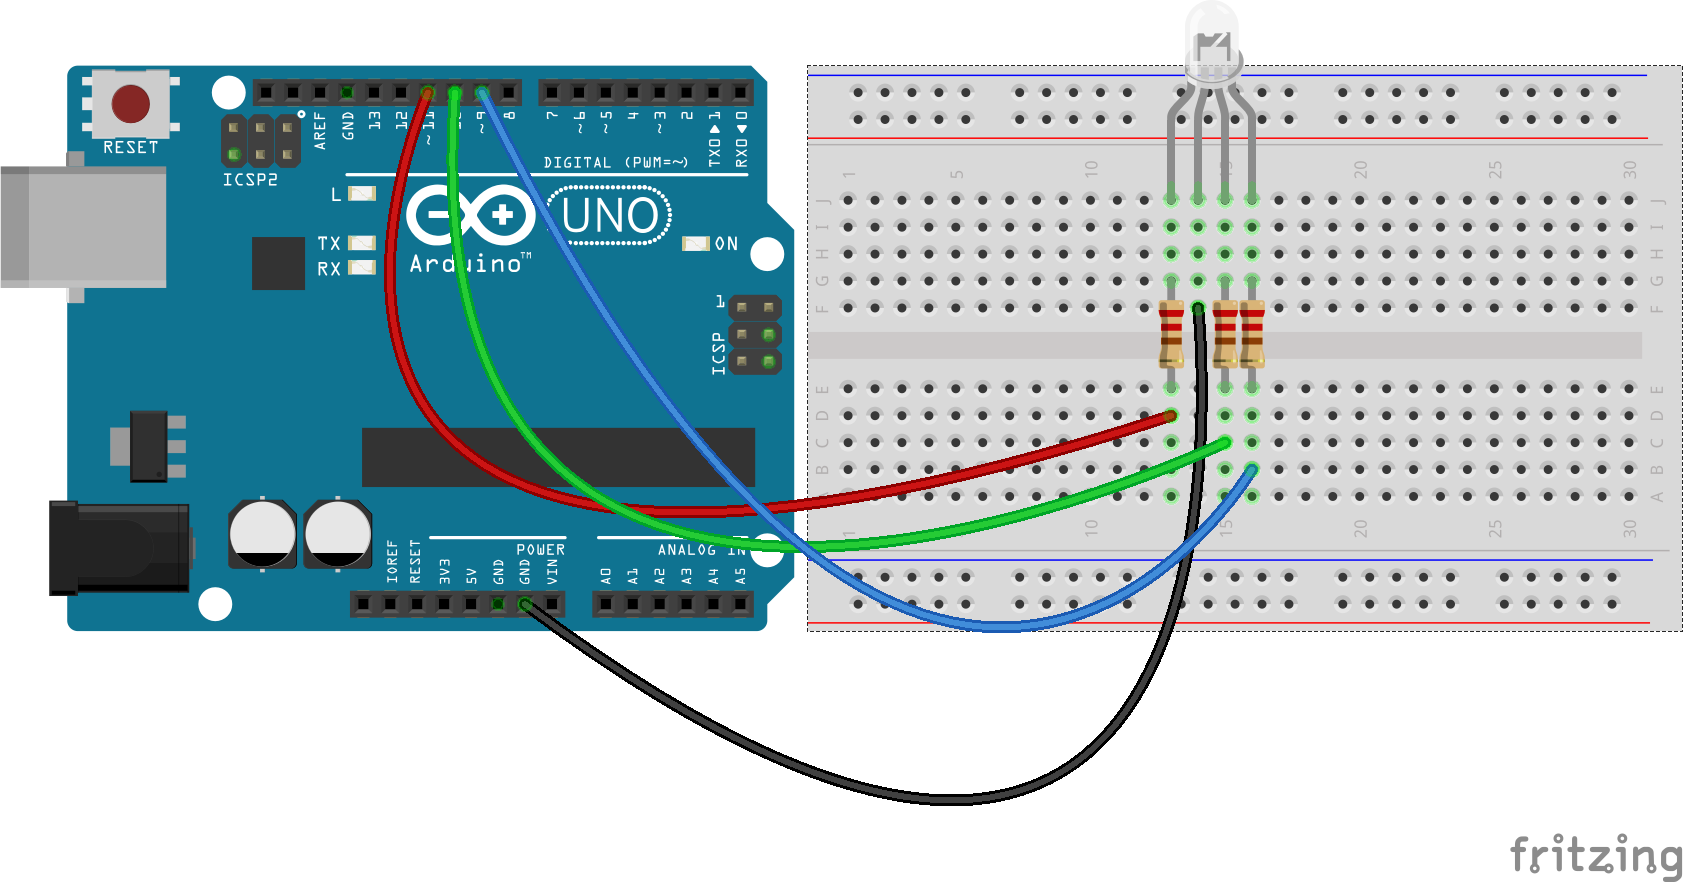
\includegraphics[width=\hgfig]{\LocLEDfig/rgb-led-bb.png}
  \caption{Interfacing an RGB LED with Arduino Uno using a breadboard}
  \label{fig:ard-rgb-bread}
\end{figure}
As shown in \figref{fig:ard-rgb-bread}, there is an RGB LED with four legs. 
From the left, the first leg represents the anode (+) pin for the red LED. 
The second leg represents the common cathode for every color. 
The third and fourth legs represent the anode (+) pins for the green LED and blue LED respectively. 
The anode pins of red, green, and blue are connected to digital pins 11, 10, and 9 of Arduino Uno, respectively. 
Common cathode is connected to the ground (GND) terminal of Arduino Uno. 

\section{Lighting the LED from the Arduino IDE}

\subsection{Lighting the LED}
\label{sec:light-ard}
In this section, we will describe some experiments that will help the
LED light up based on the command given from the Arduino IDE.  We will
also give the necessary code.  We will present four experiments in
this section.  The shield has to be attached to the \arduino\ board
before doing these experiments and the \arduino\ needs to be connected to the computer 
with a USB cable, as shown in \figref{arduino}. The reader should go through the
instructions given in \secref{sec:ard-start} before getting started.
\begin{enumerate}
  \item First, we will see how to light up the LED in different
        colours.  An extremely simple code is given in \ardref{ard:led-blue}.
        On uploading this code, you can see that the LED on the shield turns
        blue.  It is extremely easy to explain this code.  Recall from the
        above discussion that we have to put a high voltage (5V) on pin 9 to
        turn the blue light on.  This is achieved by the following command:
        \lstinputlisting[firstline=4,lastline=4]
        {\LocLEDardcode/led-blue/led-blue.ino}
        Before that, we need to define pin 9 as the
        output pin.  This is achieved by the command,
        \lstinputlisting[firstline=2,lastline=2]
        {\LocLEDardcode/led-blue/led-blue.ino}
        One can see that the blue light will be on continuously.  
        
  \item Next, we will modify the code slightly so that the blue light
        remains on for two seconds and then turns off.
        \ardref{ard:led-blue-delay} helps achieve this.  In this, we
        introduce a new command {\tt delay} as below:
        \lstinputlisting[firstline=5,lastline=5]
        {\LocLEDardcode/led-blue-delay/led-blue-delay.ino} This delay
        command halts the code for the time passed as in input argument. In
        our case, it is 2,000 milliseconds, or 2 seconds.  The next command,
        \lstinputlisting[firstline=6,lastline=6]
        {\LocLEDardcode/led-blue-delay/led-blue-delay.ino} puts a low
        voltage on pin 9 to turn it off.
        
        What is the role of the {\tt delay} command?  To find this,
        comment the delay command.  That is, replace the above delay command
        with the following and upload the code.
        \begin{lstlisting}[style=nonumbers]
    // delay(2000);
  \end{lstlisting}
        If you observe carefully, you will see that the LED turns blue
        momentarily and then turns off.
        
  \item We mentioned earlier that it was possible to light more than one
        LED simultaneously.  We will now describe this with another
        experiment.  In this, we will turn on both blue and red LEDs.  We
        will keep both of them on for 5 seconds and then turn blue off,
        leaving only red on.  After 3 seconds, we will turn red also off.
        This code is given in \ardref{ard:led-blue-red}.  Remember that
        before writing either {\tt HIGH} or {\tt LOW} on to any pin, its
        mode has to be declared as {\tt OUTPUT}, as given in the code.  All
        the commands in this code are self explanatory.
        
  \item Finally, we will give a hint of how to use the programming
        capabilities of the Arduino IDE.  For this, we will use
        \ardref{ard:led-blink}.  It makes the LED blink 5 times.  Recall
        from the previous section that a {\tt HIGH} on pin 10 turns on the
        green LED.  This cycle is executed for a total of five times.  In each
        iteration, it will turn the green LED on for a second by giving the
          {\tt HIGH} signal and then turn it off for a second by giving the
          {\tt LOW} signal.  This cycle is carried out for a total of 5 times,
        because of the {\tt for} loop.
\end{enumerate}

\paragraph{Note:}
All the above four experiments have been done with
the shield affixed to the \arduino\ board.  One may run these
experiments without the shield as well.  But in this case, pin number
13 has to be used in all experiments, as pin 13 lights up the LED that
is on the \arduino\ board.  For example, in \ardref{ard:led-blue}, one
has to replace both occurrences of number 9 with 13.  In this case,
one will get the LED of \arduino\ board light up, as shown in
\figref{fig:led-uno}.
\begin{figure}
  \centering
  \includegraphics[width=\hgfig]{\LocLEDfig/led_output.png}
  \caption{LED experiments directly on \arduino\ board, without the
    shield}
  \label{fig:led-uno}
\end{figure}


\paragraph{Note:} It should also be pointed out that only one colour
is available in \arduino\ board.  As a result, it is not possible to
conduct the experiments that produce different colours if the
shield is not used.

\begin{exercise}
  Carry out the following exercise:
  \begin{enumerate}
    \item In \ardref{ard:led-blue-delay}, remove the delay, as discussed
          above, and check what happens.
    \item Light up all three colours simultaneously, by modifying
          \ardref{ard:led-blue-red}.  Change the
          combination of colours to get different colours.
    \item Incorporate some of the features of earlier experiments into
          \ardref{ard:led-blink} and come up with different ways of blinking
          with different colour combinations.
  \end{enumerate}
\end{exercise}

\subsection{Arduino Code}
\lstset{style=mystyle}
\label{sec:led-arduino-code}
\addtocontents{ard}{\protect\addvspace{\codclr}}

\begin{ardcode}
  \acaption{Turning on the blue LED}{Turning on the blue LED.  Available
    at \LocLEDardbrief{led-blue/led-blue.ino}.}
  \label{ard:led-blue}
  \lstinputlisting{\LocLEDardcode/led-blue/led-blue.ino}
\end{ardcode}

\begin{ardcode}
  \acaption{Turning on the blue LED and turning it off after two
    seconds}{Turning on the blue LED and turning it off after two
    seconds.  Available  
    at \LocLEDardbrief{led-blue-delay/led-blue-delay.ino}.}
  \label{ard:led-blue-delay}
  \lstinputlisting{\LocLEDardcode/led-blue-delay/led-blue-delay.ino}
\end{ardcode}

\begin{ardcode}
  \acaption{Turning on blue and red LEDs for 5 seconds and then turning
    them off one by one}{Turning on blue and red LEDs for 5 seconds and
    then turning them off one by one.  Available at
    \LocLEDardbrief{led-blue-red/led-blue-red.ino}.}
  \label{ard:led-blue-red}
  \lstinputlisting{\LocLEDardcode/led-blue-red/led-blue-red.ino}
\end{ardcode}

\begin{ardcode}
  \acaption{Blinking the green LED}{Blinking the green LED.  Available
    at \LocLEDardbrief{led-green-blink/led-green-blink.ino}.}
  \label{ard:led-blink}
  \lstinputlisting{\LocLEDardcode/led-green-blink/led-green-blink.ino}
\end{ardcode}


\section{Lighting the LED from Scilab}
\subsection{Lighting the LED}
\label{sec:light-sci}
In this section, we discuss how to carry out the experiments of the
previous section from Scilab.  We will list the same four experiments,
in the same order.  The shield has to be attached to the \arduino\ board
before doing these experiments and the \arduino\ needs to be connected to the computer 
with a USB cable, as shown in \figref{arduino}.
The reader should go through the instructions given in
\secref{sec:sci-start} before getting started. 
\begin{enumerate}
  \item In the first experiment, we will light up the blue LED on the
        shield.  The code for this is given in \sciref{sci:led-blue}.  It
        begins with a command of the form
        \begin{lstlisting}[style=nonumbers]
     ok = open_serial(1, PORT NUMBER, BAUD RATE)
  \end{lstlisting}
        We have used 2 for {\tt PORT NUMBER} and 115200 for {\tt BAUD RATE}.
        As a result, this command becomes
        \lstinputlisting[firstline=1,lastline=1]{\LocLEDscicode/led-blue.sce}
        This command is used to open the serial port.  When the port is
        opened successfully, it returns a value of 0, which gets stored in
        the variable {\tt ok}.
        
        Sometimes, the serial port does not open, as mentioned in the above
        command.  This is typically due to not closing the serial port
        properly in a previous experiment.  If this condition is not
        trapped, the program will wait forever, without any information
        about this difficulty.  One way to address this difficulty is to
        terminate the program if the serial port does not open.  This is
        achieved using the error message of the following form:
        \begin{lstlisting}[style=nonumbers]
     if ok ~= 0, error(Error Message in Quotes);
  \end{lstlisting}
        It checks if {\tt ok = 0}.  If not, it flashes an error message and
        terminates.  This line gets implemented in the following way in
        \sciref{sci:led-blue}.  
        \lstinputlisting[firstline=2,lastline=2]{\LocLEDscicode/led-blue.sce}
        
        We turn the LED on in the next line.  This is achieved using a
        command of the form
        \begin{lstlisting}[style=nonumbers]
    cmd_digital_out(1, PIN NUMBER, VALUE)
  \end{lstlisting}
        As we want to turn on the blue light in the shield, as discussed in
        \secref{sec:light-ard}, we choose {\tt PIN NUMBER} as 9.  We can put
        any positive integer in the place of {\tt VALUE}.  We arrive at the
        following command:
        \lstinputlisting[firstline=3,lastline=3]{\LocLEDscicode/led-blue.sce}
        
        The last line in the code closes the serial port.  As mentioned
        above, it is extremely important to close the serial port properly.
        If not closed properly, there could be difficulties in running
        subsequent programs.
        
  \item \sciref{sci:led-blue-delay} does the same thing as what
        \ardref{ard:led-blue-delay} does.  It does two more things than what
        \sciref{sci:led-blue} does: It makes the blue LED light up for two
        seconds.  This is achieved by the command
        \lstinputlisting[firstline=4,lastline=4]{\LocLEDscicode/led-blue-delay.sce}
        The second thing this code does is to turn the blue LED off.  This
        is achieved by the command
        \lstinputlisting[firstline=5,lastline=5]{\LocLEDscicode/led-blue-delay.sce}
        It is easy to see that this code puts a 0 on pin 9.
        
  \item \sciref{sci:led-blue-red} does the same thing as what
        \ardref{ard:led-blue-red} does.  It turns blue and red LEDs on for
        five seconds.  After that, it turns off blue first.  After 3
        seconds, it turns off red also.  So, when the program ends, no LED is
        lit up.
        
  \item \sciref{sci:led-green-blink} does exactly what its counterpart
        in the Arduino IDE does.  It makes the green LED blink five times.
\end{enumerate}

\begin{exercise}
  Repeat the exercise of the previous section.
\end{exercise}

\subsection{Scilab Code}
\lstset{style=mystyle}
\label{sec:led-scilab-code}
\addtocontents{cod}{\protect\addvspace{\codclr}}

\begin{scicode}
  \ccaption{Turning on the blue LED}
  {Turning on the blue LED.  Available at
    \LocLEDscibrief{led-blue.sce}.}
  \label{sci:led-blue}
  \lstinputlisting{\LocLEDscicode/led-blue.sce}
\end{scicode}

\begin{scicode}
  \ccaption{Turning on the blue LED and turning it off after two
    seconds}{Turning on the blue LED and turning it off after two
    seconds.  Available  
    at \LocLEDscibrief{led-blue-delay.sce}.}
  \label{sci:led-blue-delay}
  \lstinputlisting{\LocLEDscicode/led-blue-delay.sce}
\end{scicode}

\begin{scicode}
  \ccaption{Turning on blue and red LEDs for 5 seconds and then turning
    them off one by one}{Turning on blue and red LEDs for 5 seconds and
    then turning them off one by one.  Available at
    \LocLEDscibrief{led-blue-red.sce}.}
  \label{sci:led-blue-red}
  \lstinputlisting{\LocLEDscicode/led-blue-red.sce}
\end{scicode}

\begin{scicode}
  \ccaption{Blinking the green LED}{Blinking the green LED.  Available
    at \LocLEDscibrief{led-green-blink.sce}.}
  \label{sci:led-green-blink}
  \lstinputlisting{\LocLEDscicode/led-green-blink.sce}
\end{scicode}


\section{Lighting the LED from Scilab Xcos}
\label{sec:light-xcos}
In this section, we will see how to light the LEDs from Scilab Xcos.
We will carry out the same four experiments as in the previous
sections.  For each, we will give the location
of the zcos file and the parameters to set.  The reader should go
through the instructions given in \secref{sec:xcos-start} before
getting started.

\begin{enumerate}
  \item First we will see how to turn on the blue LED.  When the file
        required for this experiment is invoked, one gets the GUI as in 
        \figref{fig:led-blue}.  In the caption of this figure, one can see
        where to locate the file.
        
        \begin{figure}
          \centering
          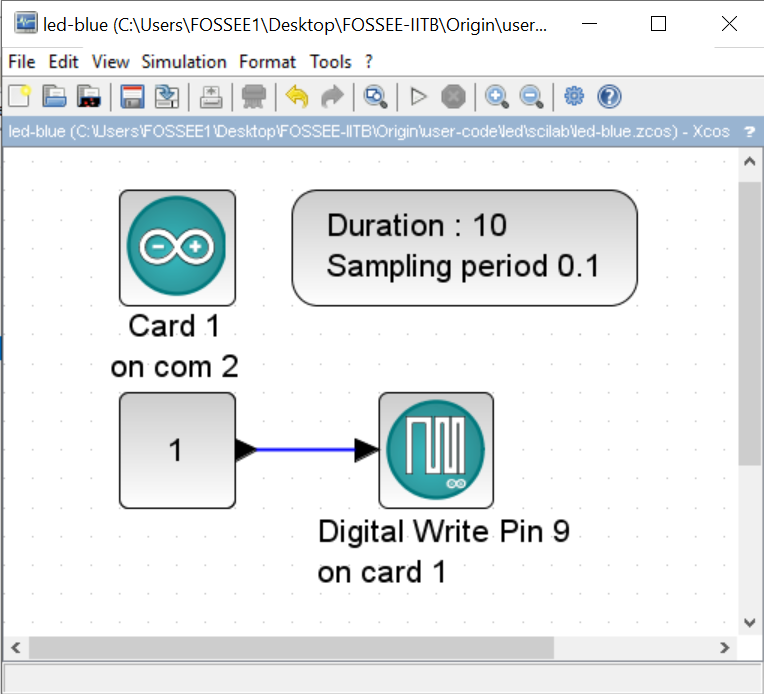
\includegraphics[width=\smfig]{\LocLEDfig/led-blue-com-2.png}
          \caption[Turning the blue LED on through Xcos]{Turning the blue
            LED on through Xcos.  This is what one sees when
            \LocLEDscibrief{led-blue.zcos} is invoked.}
          \label{fig:led-blue}
        \end{figure}
        
        We will next explain how to set the parameters for this simulation.
        To set value on any block, one needs to right click and open the
          {\tt Block Parameters} or double click.  The values for each block
        is tabulated in \tabref{tab:led-blue}.  All other parameters are to
        be left unchanged.
        \begin{table}
          \centering
          \caption{Parameters to light the blue LED in Xcos}
          \label{tab:led-blue}
          \begin{tabular}{llc} \hline
            Name of the block  & Parameter name             & Value     \\ \hline
            ARDUINO\_SETUP     & Identifier of Arduino Card & 1         \\
                               & Serial com port number     & 2\portcmd \\ \hline
            TIME\_SAMPLE       & Duration of acquisition(s) & 10        \\
                               & Sampling period(s)         & 0.1       \\ \hline
            DIGITAL\_WRITE\_SB & Digital pin                & 9         \\
                               & Arduino card number        & 1         \\ \hline
          \end{tabular}
        \end{table}
        
  \item In the second experiment, we will show how to turn on the blue LED on
        for two seconds and then to turn it off.  When the file required for
        this experiment is invoked, one gets the GUI as in
        \figref{fig:led-blue-delay}.  In the caption of this figure, one can
        see where to locate the file.
        
        \begin{figure}
          \centering
          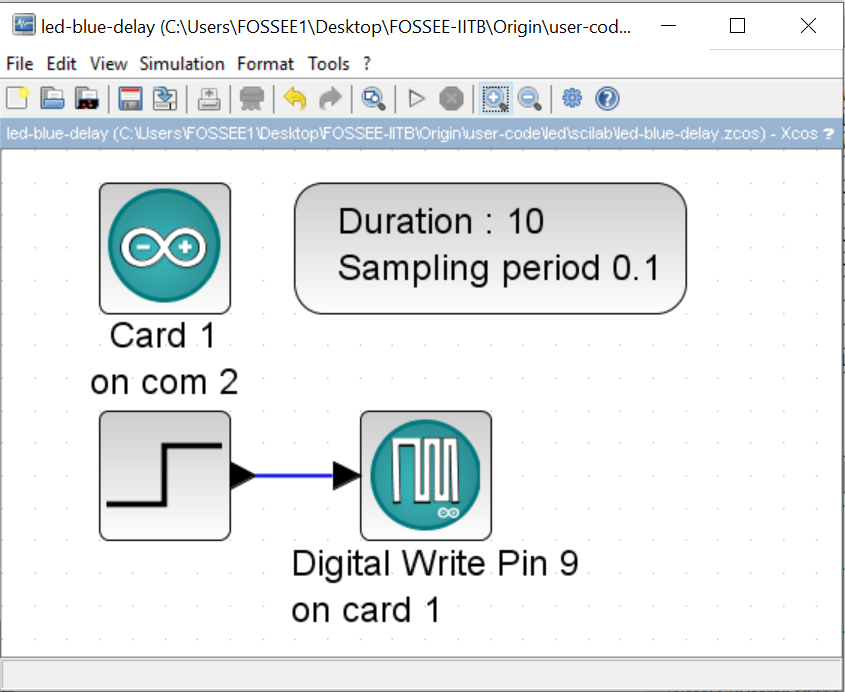
\includegraphics[width=\smfig]{\LocLEDfig/led-blue-delay-com-2.png}
          \caption[Turning the blue LED on through Xcos for two
            seconds]{Turning the blue LED on through Xcos for two
            seconds.  This is what one sees when
            \LocLEDscibrief{led-blue-delay.zcos} is invoked.}
          \label{fig:led-blue-delay}
        \end{figure}
        
        The values for each block required in this program are tabulated in
        \tabref{tab:led-blue-delay}.  All other parameters are to be left
        unchanged.
        \begin{table}
          \centering
          \caption{Parameters to light the blue LED in Xcos for two seconds}
          \label{tab:led-blue-delay}
          \begin{tabular}{llc} \hline
            Name of the block  & Parameter name             & Value     \\ \hline
            ARDUINO\_SETUP     & Identifier of Arduino Card & 1         \\
                               & Serial com port number     & 2\portcmd \\ \hline
            TIME\_SAMPLE       & Duration of acquisition(s) & 10        \\
                               & Sampling period(s)         & 0.1       \\ \hline
            DIGITAL\_WRITE\_SB & Digital pin                & 9         \\
                               & Arduino card number        & 1         \\ \hline
            STEP\_FUNCTION     & Step time                  & 2         \\
                               & Initial value              & 1         \\
                               & Final value                & 0         \\ \hline
          \end{tabular}
        \end{table}
        
  \item In the third experiment, we will show how to turn the blue LED
        and the red LED on for five seconds, turn off the blue LED and three
        seconds later, turn off the red LED also.  When the file required for
        this experiment is invoked, one gets the GUI as in
        \figref{fig:led-blue-red}.  In the caption of this figure, one can
        see where to locate the file.
        
        \begin{figure}
          \centering
          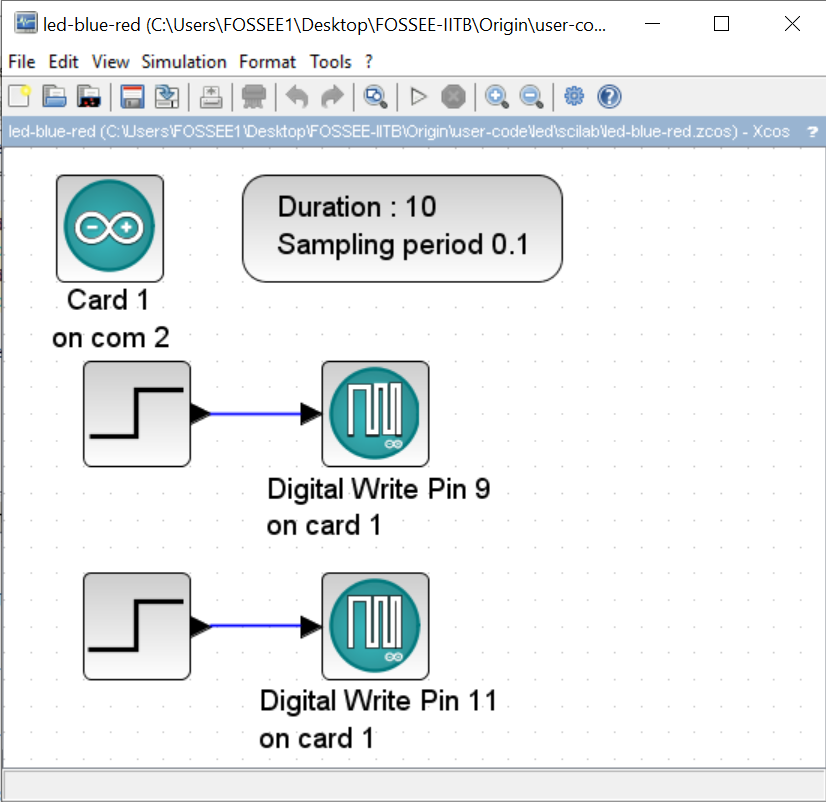
\includegraphics[width=\smfig]{\LocLEDfig/led-blue-red-com-2.png}
          \caption[Turning the blue and red LEDs on through Xcos and turning
            them off one by one]{Turning the blue and red LEDs on through
            Xcos and turning them off one by one.  This is what one sees
            when \LocLEDscibrief{led-blue-red.zcos} is invoked.}
          \label{fig:led-blue-red}
        \end{figure}
        
        The values for each block required in this program are tabulated in
        \tabref{tab:led-blue-red}.  All other parameters are to be left
        unchanged.
        \begin{table}
          \centering
          \caption{Parameters to turn the blue and red LEDs on and then turn
            them off one by one}
          \label{tab:led-blue-red}
          \begin{tabular}{llc} \hline
            Name of the block    & Parameter name             & Value     \\ \hline
            ARDUINO\_SETUP       & Identifier of Arduino Card & 1         \\
                                 & Serial com port number     & 2\portcmd \\ \hline
            TIME\_SAMPLE         & Duration of acquisition(s) & 10        \\
                                 & Sampling period(s)         & 0.1       \\ \hline
            DIGITAL\_WRITE\_SB 1 & Digital pin                & 9         \\
                                 & Arduino card number        & 1         \\ \hline
            STEP\_FUNCTION 1     & Step time                  & 5         \\
                                 & Initial value              & 1         \\
                                 & Final value                & 0         \\ \hline
            DIGITAL\_WRITE\_SB 2 & Digital pin                & 11        \\
                                 & Arduino card number        & 1         \\ \hline
            STEP\_FUNCTION 2     & Step time                  & 8         \\
                                 & Initial value              & 1         \\
                                 & Final value                & 0         \\ \hline
          \end{tabular}
        \end{table}
        
  \item We will conclude this section with an experiment to blink the
        green LED on and off.  When the file required for
        this experiment is invoked, one gets the GUI as in
        \figref{fig:led-green-blink}.  In the caption of this figure, one can
        see where to locate the file.
        
        \begin{figure}
          \centering
          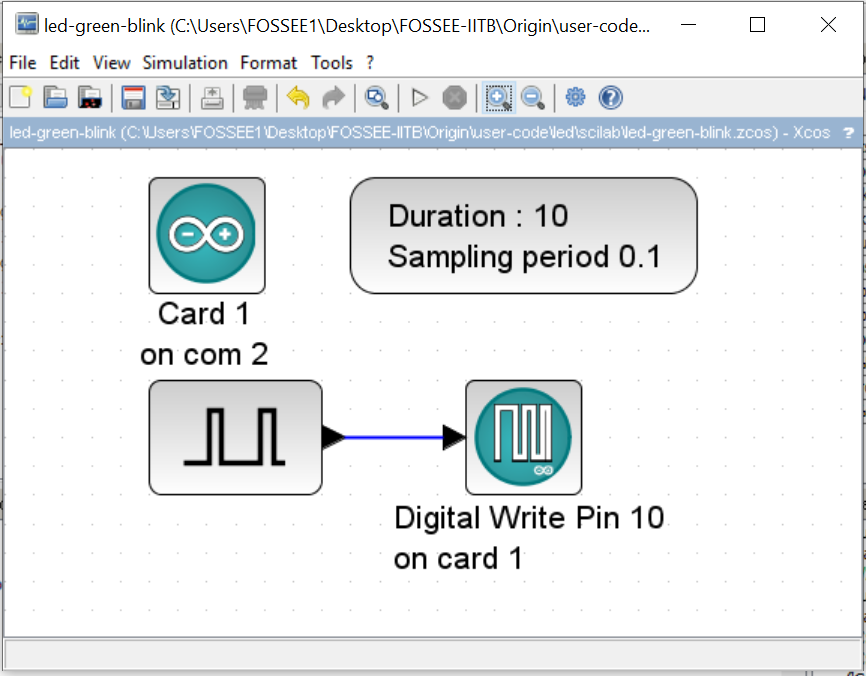
\includegraphics[width=\smfig]{\LocLEDfig/led-green-blink-com-2.png}
          \caption[Blinking the green LED every second through
            Xcos]{Blinking the green LED every second through Xcos.
            This is what one sees when
            \LocLEDscibrief{led-green-blink.zcos} is invoked.}
          \label{fig:led-green-blink}
        \end{figure}
        
        The values for each block required in this program are tabulated in
        \tabref{tab:led-green-blink}.  All other parameters are to be left
        unchanged.
        \begin{table}
          \centering
          \caption{Parameters to make the green LED blink every second}
          \label{tab:led-green-blink}
          \begin{tabular}{llc} \hline
            Name of the block  & Parameter name             & Value     \\ \hline
            ARDUINO\_SETUP     & Identifier of Arduino Card & 1         \\
                               & Serial com port number     & 2\portcmd \\ \hline
            TIME\_SAMPLE       & Duration of acquisition(s) & 10        \\
                               & Sampling period(s)         & 0.1       \\ \hline
            DIGITAL\_WRITE\_SB & Digital pin                & 10        \\
                               & Arduino card number        & 1         \\ \hline
            PULSE\_SC          & Pulse width(\% of period)  & 50        \\
                               & Period(secs)               & 2         \\ 
                               & Phase delay(secs)          & 0.1       \\
                               & Amplitude                  & 1         \\ \hline
          \end{tabular}
        \end{table}
\end{enumerate}

% \section{Control through Xcos}
% This experiment implements digital write functionality of Arduino board.
% % \begin{figure}
% % \centering
% % 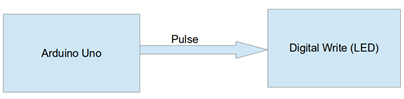
\includegraphics[width=\smfig]{\LocLEDfig/xcos-wri.png}
% % \caption{Digital write functionality}
% % \label{fig:xcoswri}
% % \end{figure}

% \begin{figure}
% \centering
% 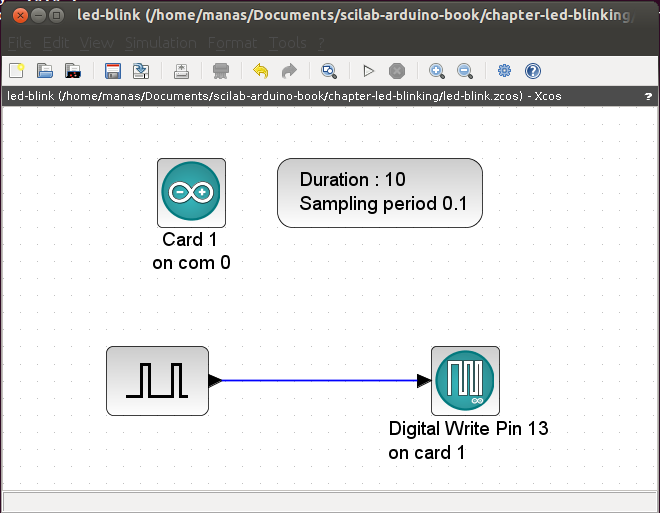
\includegraphics[width=\smfig]{\LocLEDfig/xcos-led.png}
% \caption{Xcos diagram for LED interfacing}
% \label{fig:xcosblk}
% \end{figure}

% \begin{figure}
% \centering
% 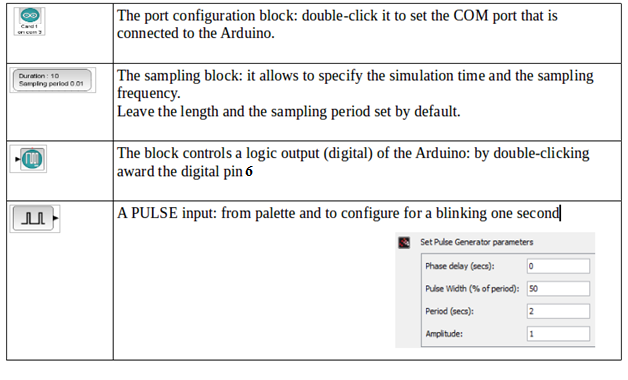
\includegraphics[width=\smfig]{\LocLEDfig/xcos-desc.png}
% \caption{Xcos blocks}
% \label{fig:xcosdesc}
% \end{figure}

% \section{Experiment: Blink LED for limited number of iterations}
% This experiment is about continuous switching on and switching off the LED a fixed number of times. Here we use  for loop to carry out limited number of iterations of the code.  The structure of for loop is:

% \begin{lstlisting}      
% for variable = start_point:end_point
%    instructions
% end
% \end{lstlisting}   

% Here variable is incremented by 1 in every iteration, till the condition variable=end\_point is met. Thus before each iteration, the above condition is verified. Figure shows the flow-chart of the operation.
% \begin{figure}
% \centering
% \includegraphics[width=\smfig]{\LocLEDfig/LEDflowchart.png}
% \caption{Flow chart}
% \label{fig:ledfc}
% \end{figure}



\begin{exercise}
  Carry out the following exercise:
  \begin{enumerate}
    \item Change the blink pattern for an array of LEDs.
    \item Change the delays.
  \end{enumerate}
\end{exercise}

\section{Lighting the LED from Python}
\subsection{Lighting the LED}
\label{sec:light-py}
In this section, we discuss how to carry out the experiments of the
previous section from Python.  We will list the same four experiments,
in the same order.  The shield has to be attached to the \arduino\ board
before doing these experiments and the \arduino\ needs to be connected to the computer 
with a USB cable, as shown in \figref{arduino}.
The reader should go through the instructions given in
\secref{sec:python-start} before getting started.
\begin{enumerate}
  \item In the first experiment, we will light up the blue LED on the
    shield.  The code for this is given in \pyref{py:led-blue}. It begins with importing 
    necessary modules, as given below: 
    \lstinputlisting[firstline=1,lastline=2]{\LocLEDpycode/led-blue.py}

    Here, {\tt os} module provides functions for interacting with the operating system. On the 
    other hand, the {\tt sys} module provides access to some variables used or maintained by the interpreter
    and functions that interact strongly with the interpreter. Next, the following lines of code are used to get the current directory 
    followed by splitting it and appending the path to {\tt PYTHONPATH} environment: 
    \lstinputlisting[firstline=3,lastline=5]{\LocLEDpycode/led-blue.py}
    
    After importing the necessary modules, following line imports the Arduino module from the Python-Arduino
    toolbox, as explained in \secref{sec:python-toolbox}:
    \lstinputlisting[firstline=7,lastline=7]{\LocLEDpycode/led-blue.py}

    Next, we will import {\tt sleep} module, which is a function available in the package pyserial \cite{pySerial}.
    For the sake of simplicity, we have configured each experiment as a class. In \pyref{py:led-blue},
    we have defined the experiment as {\tt class LED\_ON}. The following lines of code 
    initilize the parameters and functions available in this class. 
    \lstinputlisting[firstline=10,lastline=15]{\LocLEDpycode/led-blue.py}

    The function {\tt setup} creates an object of the Arduino class
    through which we can call all the methods available in the base class. 
    Along with this, it locates the port to which \arduino\ is connected 
    and opens the port for serial communication. Similar to the Scilab experiments 
    given in \secref{sec:light-sci}, we require port number and BAUD RATE for opening the serial port. 
        
        % self.obj\_arduino = Arduino() :- It creates an object of the arduino class
        % through which we can call all the methods available in the base class.Here 
        % obj\_arduino is the object created for Arduino class.Then we will call the locateport().\\
        % self.port = self.obj\_arduino.locateport() :-This method auto-detects to which port 
        % arduino is connected and assigns the port no. to the variable to self.port. Once 
        % serial port is assigned, then we will call the open\_serial() to open the serial 
        % port for communication.This is done in the next step \\
        % self.obj\_arduino.open\_serial(1, self.port,self.baudrate) :- This opens the 
        % serial port and it needs 3 parameters such as :
        
        % i. 1st arguement:- This is the board no. (1 by default) for every experiment \\
        % ii.self.port :- This is the port no. to which arduino is connected \\
        % iii.baudrate :- It sets the baudrate for serial communication \\
        
        % Then we will define the 2nd method run() in which we will define pin no. to which components are connected also apply digital or analog inputs to it depending on the digital or analog nature of the component.
    The function {\tt run} is used to define the functionality of the experiment. In this experiment, 
    we have to switch on the blue LED. For this, we define the pin number (which is 9 in this case) 
    and send the required signal to this pin. Following lines are used to implement this functionality:
    \lstinputlisting[firstline=22,lastline=24]{\LocLEDpycode/led-blue.py}

    
    At last, the function {\tt exit} is invoked to close the serial port. 
  % \item def run(self):- This method is to define the functionality of the experiment \\
  %       self.blue=9 :- pin no. to which led is connected \\
  %       self.obj\_arduino.cmd\_digital\_out(1,self.blue,1) :- As led works on digital input so we will use cmd\_digital\_out() which will switch on/off the blue colour of RGB led .
  %       This method needs 3 parameters such as : \\
  %       1st parameter:- This is the board no. (1 by default) for every experiment.
  %       2nd parameter :- pin no. to which led is connected
  %       3rd parameter :- It applies digital logic i.e. if 1, then switch on led 
  %       0, then switch off led \\
  %       Once all the functionalities are defined and the experiments are performed accordingly then we will close the serial port which  is done by the exit function.
  % \item def exit(self):- This function closes the serial port \\
        % self.obj\_arduino.close\_serial() :- this function is called from Arduino class which closes the serial port properly.
      
      Once all the parameters and functions available in {\tt class LED\_ON} have been 
      initialized, we create a main method and call it, as given below: 
      \lstinputlisting[firstline=29,lastline=33]{\LocLEDpycode/led-blue.py}

  % \item def main():- Here we will create the main method \\
  %       obj\_led=LED\_ON(115200) :- It creates an object of the class with baudrate of 115200.
  % \item if \_\_name\_\_== '\_\_main\_\_':- At last we will check for the main module
  %       whether its directly run from the file or being imported from another module \\
  %       main() :- It calls the main module and which in turn calls the object of the 
  %       class and performs the experiment.

  \item \pyref{py:led-blue-delay} does the same thing as what \ardref{ard:led-blue-delay} does. 
        It does two more things than what \pyref{py:led-blue} does: It makes the blue LED light up for two
        seconds.  This is achieved by the command
        \lstinputlisting[firstline=25,lastline=25]{\LocLEDpycode/led-blue-delay.py}
        The second thing this code does is to turn the blue LED off.  This
        is achieved by the command
        \lstinputlisting[firstline=26,lastline=26]{\LocLEDpycode/led-blue-delay.py}
        As evident, this line of code puts a 0 on pin 9.
  \item \pyref{py:led-blue-red} does the same thing as what \ardref{ard:led-blue-red} does. 
         It turns blue and red LEDs on for five seconds.  After that, it turns off blue 
         first.  After 3 seconds, it turns off red also.  So, when the program ends, 
         no LED is lit up.
  
  \item \pyref{py:led-green-blink} does exactly what its counterpart in the Arduino IDE does.  
        It makes the green LED blink five times.
\end{enumerate}

\begin{exercise}
  Repeat the exercise of the previous section.
\end{exercise}

\subsection{Python Code}
\lstset{style=mystyle}
\label{sec:led-python-code}
\addtocontents{pyd}{\protect\addvspace{\codclr}}

\begin{pycode}
  \pcaption{Turning on the blue LED}
  {Turning on the blue LED. Available at
    \LocLEDpybrief{led-blue.py}.}
  \label{py:led-blue}
  \lstinputlisting{\LocLEDpycode/led-blue.py}
\end{pycode}

\begin{pycode}
  \pcaption{Turning on the blue LED and turning it off after two
    seconds}{Turning on the blue LED and turning it off after two
    seconds.  Available  
    at \LocLEDpybrief{led-blue-delay.py}.}
  \label{py:led-blue-delay}
  \lstinputlisting{\LocLEDpycode/led-blue-delay.py}
\end{pycode}

\begin{pycode}
  \pcaption{Turning on blue and red LEDs for 5 seconds and then turning
    them off one by one}{Turning on blue and red LEDs for 5 seconds and
    then turning them off one by one.  Available at
    \LocLEDpybrief{led-blue-red.py}.}
  \label{py:led-blue-red}
  \lstinputlisting{\LocLEDpycode/led-blue-red.py}
\end{pycode}

\begin{pycode}
  \pcaption{Blinking the green LED}{Blinking the green LED.  Available
    at \LocLEDpybrief{led-green-blink.py}.}
  \label{py:led-green-blink}
  \lstinputlisting{\LocLEDpycode/led-green-blink.py}
\end{pycode}

\section{Lighting the LED from Julia}
\subsection{Lighting the LED}
\label{sec:light-julia}
In this section, we discuss how to carry out the experiments of the
previous section from Julia.  We will list the same four experiments,
in the same order.  The shield has to be attached to the \arduino\ board
before doing these experiments and the \arduino\ needs to be connected to the computer 
with a USB cable, as shown in \figref{arduino}.
The reader should go through the instructions given in \secref{sec:julia-start} before getting started.

\begin{enumerate}
  \item In the first experiment, we will light up the blue LED on the
        shield.  The code for this is given in \juliaref{julia:led-blue}.
        It begins with importing the SerialPorts \cite{julia-serial-ports} package 
        and the module ArduinoTools, as given in \secref{sec:julia-toolbox}. Following lines 
        import SerialPorts and ArduinoTools:
        \lstinputlisting[firstline=1,lastline=2]{\LocLEDjuliacode/led-blue.jl}

        Next, the following line of code is used to detect the port on which \arduino\
        is connected. 
        \lstinputlisting[firstline=4,lastline=4]{\LocLEDjuliacode/led-blue.jl}
      Apart from detecting the port, it also opens a serial port with given BAUD RATE. 
      In this experiment, we have to put a high voltage (5V) on pin 9 to
        turn the blue light on.  This is achieved by the following command:
        \lstinputlisting[firstline=6,lastline=6]{\LocLEDjuliacode/led-blue.jl}
        Before that, we need to define pin 9 as the
        output pin.  This is achieved by the following command: 
        \lstinputlisting[firstline=5,lastline=5]{\LocLEDjuliacode/led-blue.jl}
        The last line in the code closes the serial port. 
        In this Julia source file, one can observe that the blue light will be on continuously.   
\item \juliaref{julia:led-blue-delay} does the same thing as what
        \ardref{ard:led-blue-delay} does.  It does two more things than what
        \juliaref{julia:led-blue} does: It makes the blue LED light up for two
        seconds.  This is achieved by the command
      \lstinputlisting[firstline=7,lastline=7]{\LocLEDjuliacode/led-blue-delay.jl}
      The second thing this code does is to turn the blue LED off.  This
        is achieved by the command
        \lstinputlisting[firstline=8,lastline=8]{\LocLEDjuliacode/led-blue-delay.jl}
        It is easy to see that this code puts a 0 on pin 9.
  \item \juliaref{julia:led-blue-red} does the same thing as what
        \ardref{ard:led-blue-red} does.  It turns blue and red LEDs on for
        five seconds.  After that, it turns off blue first.  After 3
        seconds, it turns off red also.  So, when the program ends, no LED is
        lit up.
        
  \item \juliaref{julia:led-green-blink} does exactly what its counterpart
        in the Arduino IDE does.  It makes the green LED blink five times.
\end{enumerate}


\subsection{Julia Code}
\lstset{style=mystyle}
\label{sec:led-julia-code}
\addtocontents{juliad}{\protect\addvspace{\codclr}}

\begin{juliacode}
  \jcaption{Turning on the blue LED}
  {Turning on the blue LED.  Available at
    \LocLEDjuliabrief{led-blue.jl}.}
  \label{julia:led-blue}
  \lstinputlisting{\LocLEDjuliacode/led-blue.jl}
\end{juliacode}

\begin{juliacode}
  \jcaption{Turning on the blue LED and turning it off after two
    seconds}{Turning on the blue LED and turning it off after two
    seconds.  Available  
    at \LocLEDjuliabrief{led-blue-delay.jl}.}
  \label{julia:led-blue-delay}
  \lstinputlisting{\LocLEDjuliacode/led-blue-delay.jl}
\end{juliacode}

\begin{juliacode}
  \jcaption{Turning on blue and red LEDs for 5 seconds and then turning
    them off one by one}{Turning on blue and red LEDs for 5 seconds and
    then turning them off one by one.  Available at
    \LocLEDjuliabrief{led-blue-red.jl}.}
  \label{julia:led-blue-red}
  \lstinputlisting{\LocLEDjuliacode/led-blue-red.jl}
\end{juliacode}

\begin{juliacode}
  \jcaption{Blinking the green LED}{Blinking the green LED.  Available
    at \LocLEDjuliabrief{led-green-blink.jl}.}
  \label{julia:led-green-blink}
  \lstinputlisting{\LocLEDjuliacode/led-green-blink.jl}
\end{juliacode}



\section{Lighting the LED from OpenModelica}
\subsection{Lighting the LED}
\label{sec:light-OpenModelica}
In this section, we discuss how to carry out the experiments of the
previous section from OpenModelica.  We will list the same four experiments,
in the same order.  The shield has to be attached to the \arduino\ board
before doing these experiments and the \arduino\ needs to be connected to the computer 
with a USB cable, as shown in \figref{arduino}.
The reader should go through the instructions given in
\secref{sec:OpenModelica-start} before getting started.

\begin{enumerate}
  \item In the first experiment, we will light up the blue LED on the
        shield.  The code for this is given in \OpenModelicaref{OpenModelica:led-blue}.
        It begins with importing the two packages: Streams and SerialCommunication from the toolbox, as 
        given in \secref{sec:load-om-toolbox}. Following line imports this package: 
        \lstinputlisting[firstline=3,lastline=4]{\LocLEDOpenModelicacode/led-blue.mo}

    We define some variables to collect the results coming from different functions. Following 
    lines are used for these:
    \lstinputlisting[firstline=5,lastline=7]{\LocLEDOpenModelicacode/led-blue.mo}

    Now, we have a command of the form 
        \begin{lstlisting}[style=nonumbers]
     ok := sComm.open_serial(1, PORT NUMBER, BAUD RATE)
  \end{lstlisting}
        We have used 2 for {\tt PORT NUMBER} and 115200 for {\tt BAUD RATE}.
        As a result, this command becomes 
        \lstinputlisting[firstline=10,lastline=10]{\LocLEDOpenModelicacode/led-blue.mo}
        This command is used to open the serial port.  When the port is
        opened successfully, it returns a value of 0, which gets stored in
        the variable {\tt ok}.
        
        Sometimes, the serial port does not open, as mentioned in the above
        command.  This is typically due to not closing the serial port
        properly in a previous experiment.  If this condition is not
        trapped, the program will wait forever, without any information
        about this difficulty.  One way to address this difficulty is to
        terminate the program if the serial port does not open.  This is
        achieved using the error message of the following form:
        \begin{lstlisting}[style=nonumbers]
            if ok <> 0 then strm.print(Error Message in Quotes);
        \end{lstlisting}

        We turn the LED on in the upcoming lines.  This is achieved using a
        command of the form
        \begin{lstlisting}[style=nonumbers]
          digital_out := sComm.cmd_digital_out(1, PIN NUMBER, VALUE)
  \end{lstlisting}
        As we want to turn on the blue light in the shield, as discussed in
        \secref{sec:light-ard}, we choose {\tt PIN NUMBER} as 9.  We can put
        any positive integer in the place of {\tt VALUE}.  We arrive at the
        following command:
        \lstinputlisting[firstline=15,lastline=15]{\LocLEDOpenModelicacode/led-blue.mo}
        Subsequently, we close the serial port and then define the simulation parameters. 
  \item \OpenModelicaref{OpenModelica:led-blue-delay} does the same thing as what
        \ardref{ard:led-blue-delay} does.  It does two more things than what
        \OpenModelicaref{OpenModelica:led-blue} does: It makes the blue LED light up for two
        seconds.  This is achieved by the command
        \lstinputlisting[firstline=16,lastline=16]{\LocLEDOpenModelicacode/led-blue-delay.mo}
        The second thing this code does is to turn the blue LED off.  This
        is achieved by the command
        \lstinputlisting[firstline=17,lastline=17]{\LocLEDOpenModelicacode/led-blue-delay.mo}
        It is easy to see that this code puts a 0 on pin 9.
        
  \item \OpenModelicaref{OpenModelica:led-blue-red} does the same thing as what
        \ardref{ard:led-blue-red} does.  It turns blue and red LEDs on for
        five seconds.  After that, it turns off blue first.  After 3
        seconds, it turns off red also.  So, when the program ends, no LED is
        lit up.
        
  \item \OpenModelicaref{OpenModelica:led-green-blink} does exactly what its counterpart
        in the Arduino IDE does.  It makes the green LED blink five times.
  \end{enumerate}

\subsection{OpenModelica Code}
Unlike other code files, the code/ model for running experiments using OpenModelica are 
available inside the OpenModelica-Arduino toolbox, as explained in \secref{sec:load-om-toolbox}.
Please refer to \figref{om-examples-toolbox} to know how to locate the experiments. 
\lstset{style=mystyle}
\label{sec:led-OpenModelica-code}
\addtocontents{OpenModelicad}{\protect\addvspace{\codclr}}

\begin{OpenModelicacode}
  \mcaption{Turning on the blue LED}
  {Turning on the blue LED. Available at Arduino -> SerialCommunication -> 
  Examples -> led -> led\_blue.}
  \label{OpenModelica:led-blue}
  \lstinputlisting{\LocLEDOpenModelicacode/led-blue.mo}
\end{OpenModelicacode}

\begin{OpenModelicacode}
  \mcaption{Turning on the blue LED and turning it off after two
    seconds}{Turning on the blue LED and turning it off after two
    seconds.  Available at Arduino -> SerialCommunication -> Examples -> led 
    -> led\_blue\_delay.}
  \label{OpenModelica:led-blue-delay}
  \lstinputlisting{\LocLEDOpenModelicacode/led-blue-delay.mo}
\end{OpenModelicacode}

\begin{OpenModelicacode}
  \mcaption{Turning on blue and red LEDs for 5 seconds and then turning
    them off one by one}{Turning on blue and red LEDs for 5 seconds and
    then turning them off one by one.  Available at Arduino -> SerialCommunication -> Examples -> led -> led\_blue\_red.}
  \label{OpenModelica:led-blue-red}
  \lstinputlisting{\LocLEDOpenModelicacode/led-blue-red.mo}
\end{OpenModelicacode}

\begin{OpenModelicacode}
  \mcaption{Blinking the green LED}{Blinking the green LED.  Available at Arduino -> SerialCommunication -> Examples -> led -> led\_green\_blink.}
  \label{OpenModelica:led-green-blink}
  \lstinputlisting{\LocLEDOpenModelicacode/led-green-blink.mo}
\end{OpenModelicacode}

%%%%%end OpenModelicamo
